
\section{Recursive neural network models} \label{methods}

We study neural models that adhere to the linguistic \ii{principle of
 compositionality}, which says that the meanings for complex
expressions are derived from the meanings of their constituent parts
via specific composition functions \cite{Partee84,Janssen97}. In our
distributed setting, word meanings are vectors of length $n$. The
composition function maps pairs of them to single vectors of length $n$, 
which can then be merged again to represent more complex
phrases. Once the entire sentence-level representation has been
derived, it serves as a fixed-length input for some subsequent function.

We use the model architecture proposed in \cite{bowman2013can} and
depicted in Figure~\ref{sample-figure}. The two phrases being compared
are built up separately on each side of the tree, using the same
composition function, until they have each been reduced to single
vectors. The resulting vectors are fed into a separate comparison
layer that is meant to generate a feature vector capturing the
label between the two phrases. The output of this layer is then
given to a softmax classifier, which in turn produces a hypothesized
distribution over the seven labels represented in Table~\ref{b-table}.


For a composition layer, we evaluate models with both the plain neural
network layer function \eqref{rnn} and the RNTN layer function
\eqref{rntn} proposed in \citet{chen2013learning}. A sigmoid
nonlinearity (element-wise $\tanh$) is applied to the output of either
layer function, following \cite{socher2013acl1}.
%
\begin{gather} \label{rnn}
\vec{y}_{\textit{RNN}} = f(\mathbf{M} [\vec{x}^{(l)}; \vec{x}^{(r)}] + \vec{b}) \\ % TODO: Add column vectors?
\label{rntn}
\vec{y}_{\textit{RNTN}} = f(\vec{x}^{(l)T} \mathbf{T}^{[1 \ldots n]} \vec{x}^{(r)} + \mathbf{M} [\vec{x}^{(l)}; \vec{x}^{(r)}] + \vec{b})
\end{gather} 
%
Here, $\vec{x}^{(l)}$ and $\vec{x}^{(r)}$ are the column vector
representations for the left and right children of the node, and
$\vec{y}$ is the node's output.  The RNN concatenates them, multiplies
them by an $n \times 2n$ matrix of learned weights, and applies the
element-wise non-linearity to the resulting vector. The RNTN has the
same basic structure, but with the addition of a learned third-order
tensor $\mathbf{T}$, dimension $n \times n \times n$, modeling
multiplicative interactions between the child vectors. Both models
include a bias vector~$\vec{b}$.

The comparison layer uses the same kind of function template as the
composition layers (either an NN layer or an NTN layer) with
independently learned parameters and a separate nonlinearity function.
Rather than use a $\tanh$ nonlinearity here, we follow \cite{bowman2013can} 
in using a rectified linear function. In
particular, we use the leaky rectified linear function
\cite{maasrectifier}: $f(\vec{x})=\max(\vec{x}, 0) +
0.01\min(\vec{x}, 0)$, applied element-wise.

To run the model forward and label a pair of phrases, the structure of
the lower layers of the network is assembled so as to mirror the tree
structures provided for each phrase. The word vectors are then looked
up from the vocabulary matrix $V$ (one of the model parameters), and
the composition and comparison functions are used to pass information
up the tree and into the classifier at the top. For an objective
function, we use the negative log of the probability assigned to the
correct label.

% Removed 'minibatch' -> For two of the experiments, we use minibatches
% of size 1, which doesn't really count.
We train the model using stochastic gradient descent (SGD)
with learning rates computed using AdaGrad \cite{duchi2011adaptive}.
The parameters (including the vocabulary) are initialized randomly 
using a uniform distribution over $[-0.1, 0.1]$.
Because the seven classes are not balanced in general, we report performance
using both accuracy and macroaveraged F1, since the latter emphasizes
 performance on infrequent classes. We compute macroaveraged F1 
as the harmonic mean of mean precision and mean recall, both computed
for all classes for which there is test data, setting precision to 0 
where it is not defined. Source code and generated data will be released
after the review period.

\begin{figure}[tp]
  \centering
 % \includegraphics[scale=0.35]{model.eps}
  \begin{subfigure}[t]{0.45\textwidth}
\centering
\scalebox{0.75}{
 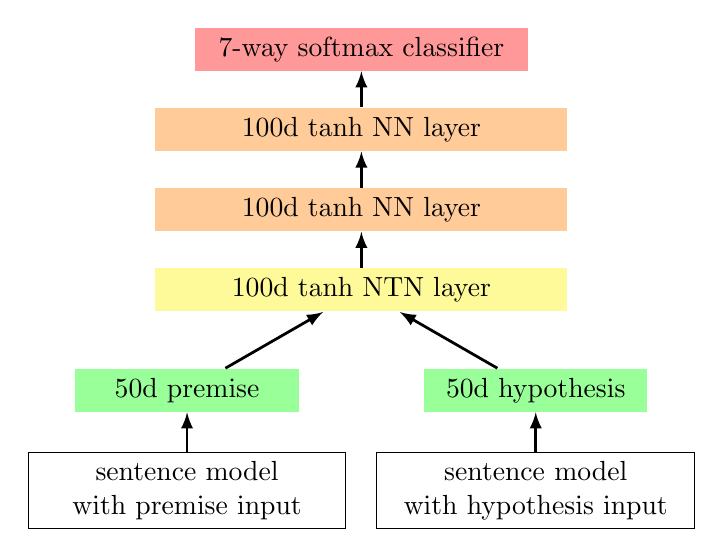
\begin{tikzpicture}
    \def\dx{21pt}
    \def\dy{29pt}

    \tikzstyle{label}=[text width=40mm,align=center]    
    \tikzstyle{softmax}=[fill=red!40,text width=40mm,align=center]
    \tikzstyle{preclass}=[fill=orange!40,text width=50mm,align=center]
    \tikzstyle{e}=[fill=green!40,text width=26mm,align=center]
    \tikzstyle{m}=[draw=black,text width=38mm,align=center]    
    
    \node[softmax]  (softmax) at (0*\dx,6*\dy) {7-way softmax classifier};
    \node[preclass]  (pc3) at (0*\dx,5*\dy) {100d $\tanh$ NN layer};
    \node[preclass]  (pc2) at (0*\dx,4*\dy) {100d $\tanh$ NN layer};
    \node[preclass,fill=yellow!40]  (pc1) at (0*\dx,3*\dy) {100d $\tanh$ NTN layer};
    \node[e]  (pe) at (-3*\dx,1.75*\dy) {50d premise};
    \node[e]  (he) at (3*\dx,1.75*\dy) {50d hypothesis};
    \node[m]  (pem) at (-3*\dx,0.5*\dy) {sentence model\\ with premise input};
    \node[m]  (hem) at (3*\dx,0.5*\dy) {sentence model\\ with hypothesis input};    
    
    \pgfsetarrowsend{latex}
    \tikzstyle{fwd} = [draw=black, line width=1pt]

          \draw [fwd] (pc3) -- (softmax);
          \draw [fwd] (pc2) -- (pc3);
          \draw [fwd] (pc1) -- (pc2);
          \draw [fwd] (pe) -- (pc1);
          \draw [fwd] (he) -- (pc1);
          \draw [fwd] (hem) -- (he);
          \draw [fwd] (pem) -- (pe);

  \end{tikzpicture}}
  
 \caption{The general architecture shared across models.}\label{fig:model:top}
  
\end{subfigure}

\begin{subfigure}[t]{0.45\textwidth}
  \centering
\scalebox{0.75}{
 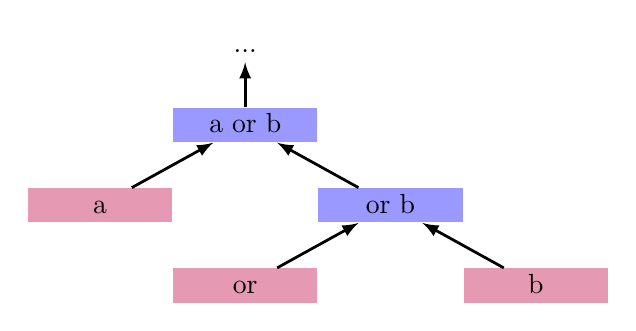
\begin{tikzpicture}
    \def\dx{21pt}
    \def\dy{29pt}


    \tikzstyle{word}=[fill=purple!40,text width=16mm,text height=2mm,align=center]
    \tikzstyle{node}=[fill=blue!40,text width=16mm,text height=2mm,align=center]
    \tikzstyle{empty}=[fill=blue!0,text width=8mm,text height=2mm,align=center]

    \node[empty]  (null) at (0*\dx,7*\dy) {...};
    \node[node]  (aorb) at (0*\dx,6*\dy) {a or b};
    \node[word]  (a) at (-2.5*\dx,5*\dy) {a};
    \node[node]  (orb) at (2.5*\dx,5*\dy) {or b};
    \node[word]  (or) at (0*\dx,4*\dy) {or};
    \node[word]  (b) at (5*\dx,4*\dy) {b};
    
    
    \pgfsetarrowsend{latex}
    \tikzstyle{fwd} = [draw=black, line width=1pt]

          \draw [fwd] (or) -- (orb);
          \draw [fwd] (b) -- (orb);
          \draw [fwd] (a) -- (aorb);
          \draw [fwd] (orb) -- (aorb);
          \draw [fwd] (aorb) -- (null);
  \end{tikzpicture}}
  
     \caption{The architecture for the TreeRNN and TreeRNTN sentence models. Terminal nodes are learned embeddings and nonterminal nodes are either NN or NTN layers with $\tanh$ nonlinearities.}\label{fig:model:tree}
  
  \end{subfigure}
 \vspace{0.5cm}
  
\begin{subfigure}[t]{0.45\textwidth}
  \centering
\scalebox{0.75}{
 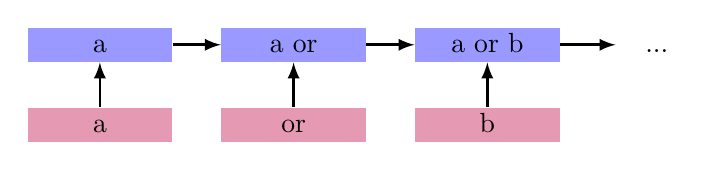
\begin{tikzpicture}
    \def\dx{35pt}
    \def\dy{29pt}


    \tikzstyle{word}=[fill=purple!40,text width=16mm,text height=2mm,align=center]
    \tikzstyle{node}=[fill=blue!40,text width=16mm,text height=2mm,align=center]
    \tikzstyle{empty}=[fill=blue!0,text width=8mm,text height=2mm,align=center]

    \node[word]  (a) at (-3*\dx,1*\dy) {a};
    \node[node]  (aN) at (-3*\dx,2*\dy) {a};
    
    \node[word]  (or) at (-1*\dx,1*\dy) {or};
    \node[node]  (orN) at (-1*\dx,2*\dy) {a or};
    
    \node[word]  (b) at (1*\dx,1*\dy) {b};
    \node[node]  (bN) at (1*\dx,2*\dy) {a or b}; 
    
    \node[empty]  (nullN) at (2.75*\dx,2*\dy) {...}; 
    
    \pgfsetarrowsend{latex}
    \tikzstyle{fwd} = [draw=black, line width=1pt]

          \draw [fwd] (or) -- (orN);
          \draw [fwd] (b) -- (bN);
          \draw [fwd] (a) -- (aN);
          \draw [fwd] (aN) -- (orN);
          \draw [fwd] (orN) -- (bN);
          \draw [fwd] (bN) -- (nullN);
          
  \end{tikzpicture}}
  
   \caption{The architecture for the LSTM sentence model. Nodes in the lower row are learned embeddings and nodes on the upper row are LSTM units.}\label{fig:model:seq}
  
    \end{subfigure}
  \caption{The model structure used to compare \ii{((all reptiles) walk)} and \ii{((some turtles) move)}. 
    The same structure is used for both the RNN and RNTN layer functions.} 
  \label{sample-figure}
\end{figure}


%\ii{Source code and generated data will be released after the conclusion of the review period.} % TODO: Or upon request? Attach anonymized code?

